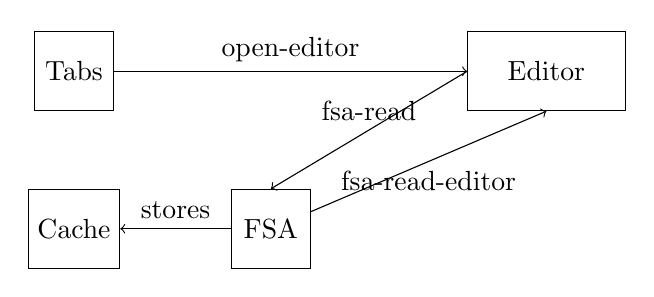
\begin{tikzpicture}
    \node (tabs) [rectangle, draw, minimum height=1cm, minimum width=1cm] at (0, 1) {Tabs};
    \node (editor) [rectangle, draw, minimum height=1cm, minimum width=2cm] at (6, 1) {Editor};
    \node (fsa) [rectangle, draw, minimum height=1cm, minimum width=1cm] at (2.5, -1) {FSA};
    \node (cache) [rectangle, draw, minimum height=1cm, minimum width=1cm] at (0, -1) {Cache};

    \draw[->] (tabs) to node[midway, above] {open-editor} (editor);
    \draw[->] (editor.west) to node[midway, above] {fsa-read} (fsa.north);
    \draw[->] (fsa) to node[midway, below] {fsa-read-editor} (editor.south);
    \draw[->] (fsa) to node[midway, above] {stores} (cache);
\end{tikzpicture}
